\section{Data Set}
% DEBS 2019  Challenge provides training and test data sets which are well-described in \cite{DEBSGC2019}.
% Here we provided a brief overview of the data set.
The data set consist of a LiDAR sensor point cloud which has 64 lasers. Each scene includes 72,000 data readings
which include X, Y, and Z coordinates (Y-axis is shown to be the elevation).
In each scene, objects are placed around the LiDAR scanner and point cloud data is collected.

% Example objects are \textbf{ATM machine}, \textbf{pedestrian}, \textbf{benches}, \textbf{cloth recycling container}.

We generated multiple 2D and 3D visualizations of the data like shown in Figures \ref{fig:ground_before},  \ref{fig:after}
and \ref{fig:ClusteringWithNoiseFiltering} to explore the data set.
Additionally, we generated animated images of the sequences of scenes to check if the scene sequences have any relations to each other.
We observed that the sequence of scenes has no relations and scenes are randomly selected from a set of scenes. Each scene includes a set of a different object placed around the LiDAR scanner.

However, in real-world applications like autonomous vehicles, sequences of scenes are correlated in their time-sequence so that
one can track the object coming in a range of LiDAR laser and going out of the view range.
The sequence information could be used to improve the classification accuracy if the correlation between scenes exists.



% SAEED
% The data provided for the challenge consists of point cloud readings simulated for a LiDAR sensor that mounts 64 lasers Fig.\ref{fig:data_overview} a , each shoot 1125 times per rotation. That is, each scene consists of 72,000 readings. Each reading is composed of attributes where X, Y, and Z coordinates are as presented in Fig.\ref{fig:data_overview} b.
%
% In each scene, objects are representative of urban environments and are of the following types: \textbf{ATM machine}, \textbf{pedestrian}, \textbf{benches}, \textbf{cloth recycling container}, \textbf{drinking fountain}, \textbf{electrical cabinet}, \textbf{emergency phone}, \textbf{fire hydrant}, \textbf{glass recycling container}, \textbf{ice freeze container}, \textbf{mailbox}, \textbf{trash bins}, \textbf{phone booth}, \textbf{trees}, and \textbf{several vehicle types}. In some cases, it is possible for an object in a scene to be hidden from the LiDAR sensor (e.g., when such object is occluded by other objects in the scene)\cite{DEBSGC2019}.


%
% \begin{figure*}[!ht]
% \begin{center}
%   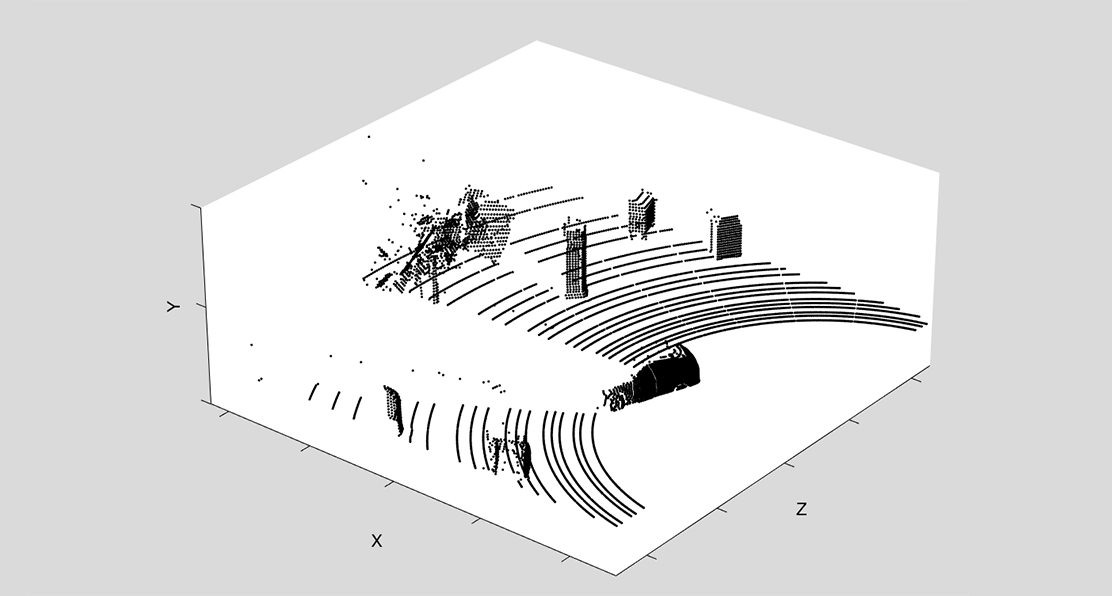
\includegraphics[width=0.8\textwidth]{./images/GC1.png}
%   \caption{An Overview of Data Set from Point Cloud of a single Scene}
%   \label{fig:data_overview}
% \end{center}
% \end{figure*}

%\usepackage{graphics} is needed for \includegraphics


% \begin{figure}%
%     \centering
%     \subfloat[point cloud readings simulated for a LiDAR sensor]{{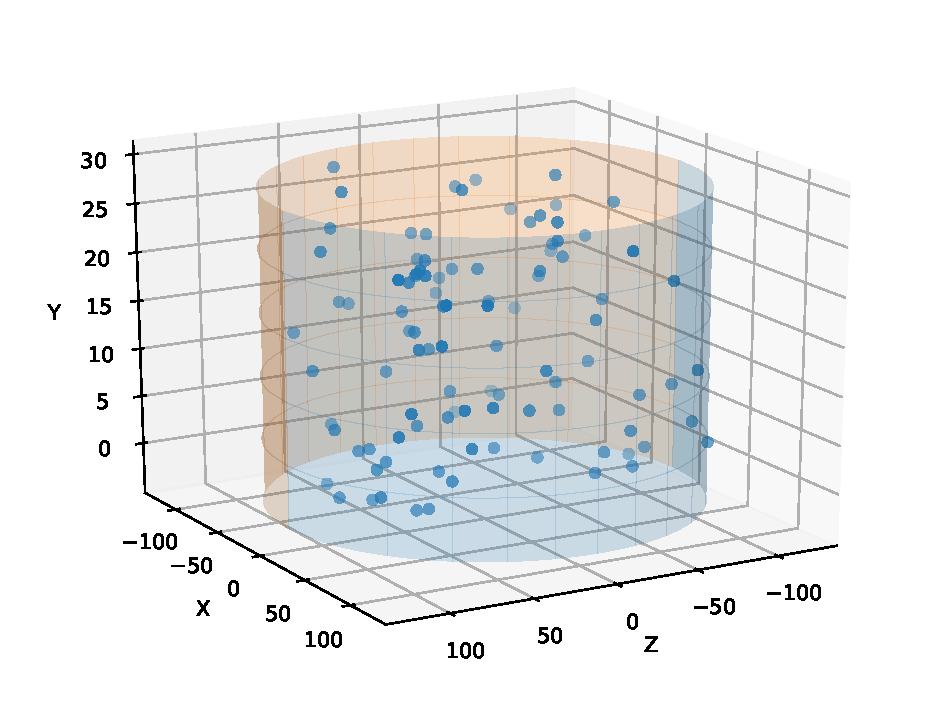
\includegraphics[width=7cm]{images/data_overview.pdf} }}%
%     \qquad
%     \subfloat[a scene with different numbers of objects]{{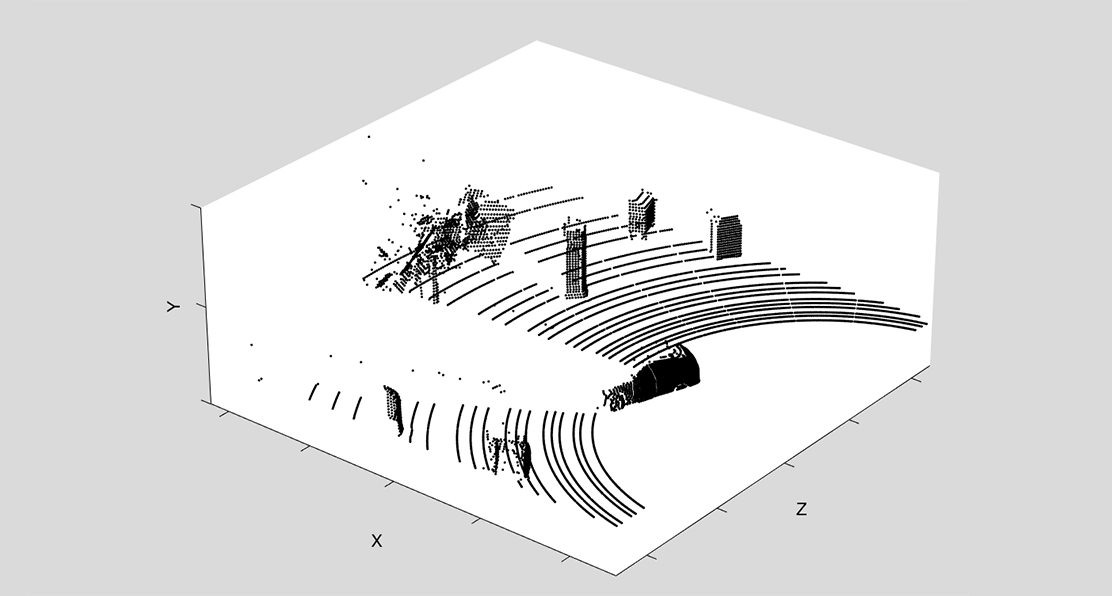
\includegraphics[width=5cm]{images/GC1.png} }}%
%     \caption{An Overview of Data Set from Point Cloud of a single Scene}%
%     \label{fig:data_overview}%
% \end{figure}


%KIA
%Briefly describe the data set and cite the main grand challenge paper.

%We just need to describe what the data is about.

% We need to mention other data sets like The KITTI Dataset \cite{Geiger2013IJRR}


% KITTI Dataset \cite{Geiger2013IJRR}
